Throughout this thesis, the logistic model for the Alaskan brown bear population will be of the form,
\begin{equation}\label{eq:LogBear}
    \frac{dy}{dt} = r_yy\left(1-\frac{y}{K_y}\right).
\end{equation}
Researchers Lawrence J. Van Daele and Victor G. Barnes Jr. wrote a report ``MANAGEMENT OF BROWN BEAR HUNTING ON KODIAK ISLAND, A\-L\-A\-S\-K\-A'' in 2010 that discusses the growth of the brown bear population and harvest strategies to maintain a healthy species~\cite{daele2010management}.
They collected data using aerial surveys in Kodiak Archipelago and developed a deterministic population model using RISKMAN, a RISK MANagement Decision Tool~\cite{daele2010management,deterministic}. From the model, they approximated a growth rate of $\lambda=1.014$ for Kodiak bears.
So, we estimate $r_y=\ln(1.014)\approx0.014$ to be the stochastic growth rate for Barnes' and Van Daele's deterministic model.
% According to Barnes' and Van Deale's analysis of their deterministic population model, the growth rate of the Alaskan brown bear population should be $r_y = 0.014$~\cite{daele2010management}.

% Now, according to the Alaska Fish \& Game Department (ADFG), the current recorded population for brown bears is estimated to be 30,000 \cite{ADFG}.
% The population shouldn't reach more than 40,000 to 50,000 due to environmental control, so it seems fair to keep the carry capacity around there \cite{ADFG}. 
% 
% From the data collected by \cite{wielgus1994dynamics,daele2010management} a graph below is produced.
% \begin{figure}[H]
%     \centering
%     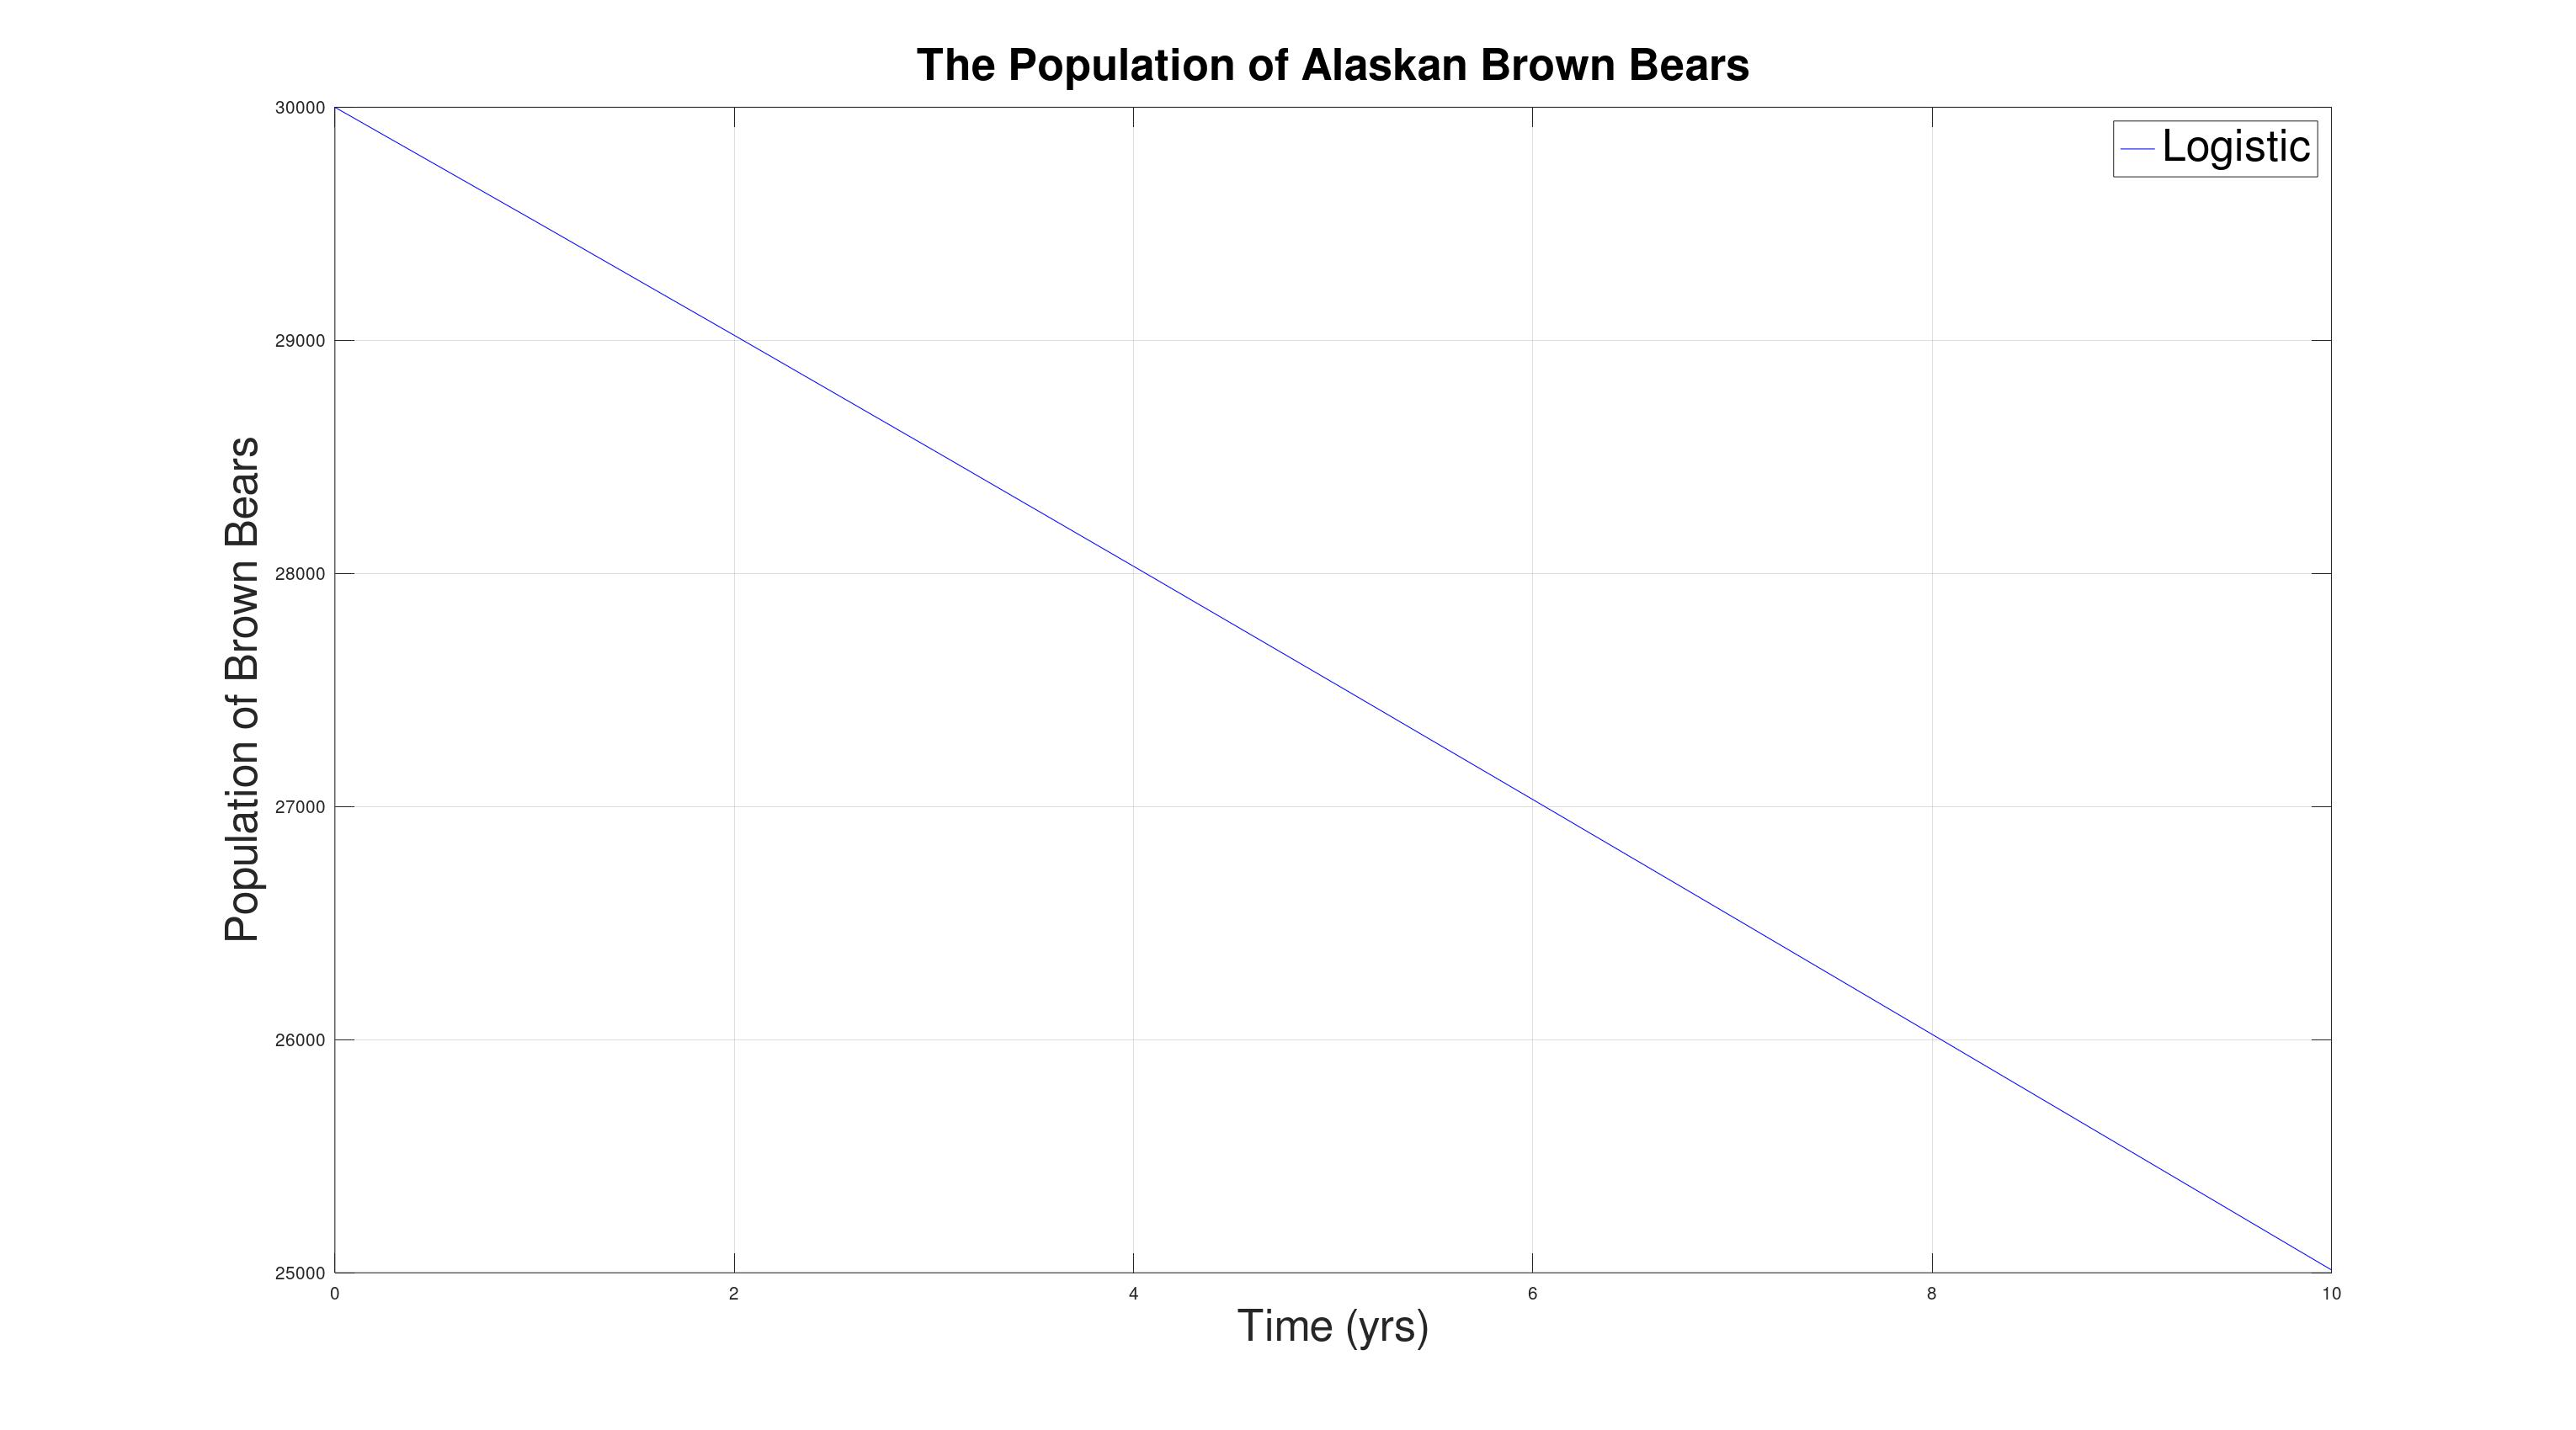
\includegraphics[width=14cm, height=8cm]{Pictures/Population_daele.jpg}
%     \caption{Using the combined data from the Van Daele's and Wielgus' articles, we can plot a prediction of the Alaskan brown bear population after 10 years\cite{daele2010management,wielgus1994dynamics}. The population decreases by 16.63\% over those 10 years.}
%     \label{fig:PopVD}
% \end{figure}
% From this graph we can see that the population is definitely decreasing over time. The end predicted population after 10 years is 25,012 which implies a 16.63\% decrease in population over that time frame. While \cite{daele2010management} seemed to have predicted an increase in population, the construction of their model isn't available to compare against. Van Daele and Barnes did compare their result to other article and found similar results produce by the basic logistic growth model, \equationautorefname~\eqref{eq:basicgrowth} \cite{daele2010management}. From Van Daele and Barnes discussion models ranged from about 16.6\% increase over 10 years and a 19\% decrease over 11 years\cite{daele2010management}. A reason for the difference in population growth could be the area the data was collected in.
% \\

% An article that is similar to Barnes' and Van Daele's management report was produced by Robert B. Wielgus and Fred L. Bunnell that investigated the growth rate of brown bears in Kananaskis Park and Bow Crow Forest of 
% southwestern Alberta, Canada~\cite{wielgus1994dynamics}.
% Wielgus and Bunnell collected their data by trapping and placing collars on their sample.
% Once the survival and reproduction rate was estimated from the data, they implemented the Lotka-Volterra equation to approximate their growth rate $r_y = \pm 0.01$.

Van Daele and Barnes compare their results to Bruce N. McLellan's research on the dynamics of grizzly bears.
McLellan's article, ``Dynamics of a grizzly bear population during a period of industrial resource extraction. III. Natality and rate of increase,'' used the Lotka equation to estimate the growth rate of a grizzly bear population in Flathead Valley, British Columbia from 1979 to 1989~\cite{mclellan1989}.
In this article, McLellan achieves an estimated growth rate of $r_y=0.081$.
In another article, ``Estimating population growth of grizzly bears from the Flathead River drainage using computer simulations of reproduction and survival rates,'' Frederick W. Hovey and Bruce N. McLellan have continued the research, now from 1979 to 1994, in Flathead Valley and chose a different method of estimating the growth rate on the extended data~\cite{mclellan1996}.
Hovey and McLellan used the bootstrap method to improve the accuracy of estimating bias and standard error compared to the method used in McLellan's 1989 article.
With the new method of calculating the growth rate and the increase in data size, Mclellan and Hovey have found similar results to Mclellan's 1989 article, where the newfound growth rate is $r_y=0.082$.

Before comparing these growth rates, a carrying capacity for the brown bear population needs to be estimated.
According to the Alaska Fish \& Game Department (ADFG), the current recorded population of brown bears is estimated to be 30,000 \cite{ADFG}.
From all the articles above, the common consensus is that the ADFG would like to maintain the size of the Alaskan bear population and keep it from climbing much higher than it is currently~\cite{mclellan1989,mclellan1996,daele2010management}.
For this reason, a carrying capacity of $K_y=45,000$ would be an appropriate estimation of the brown bears' environmental size limit.
Now, for comparison, the graphs below display the solutions of \equationautorefname~\eqref{eq:LogBear} for each growth rate.
\begin{figure}[H]
    \centering
    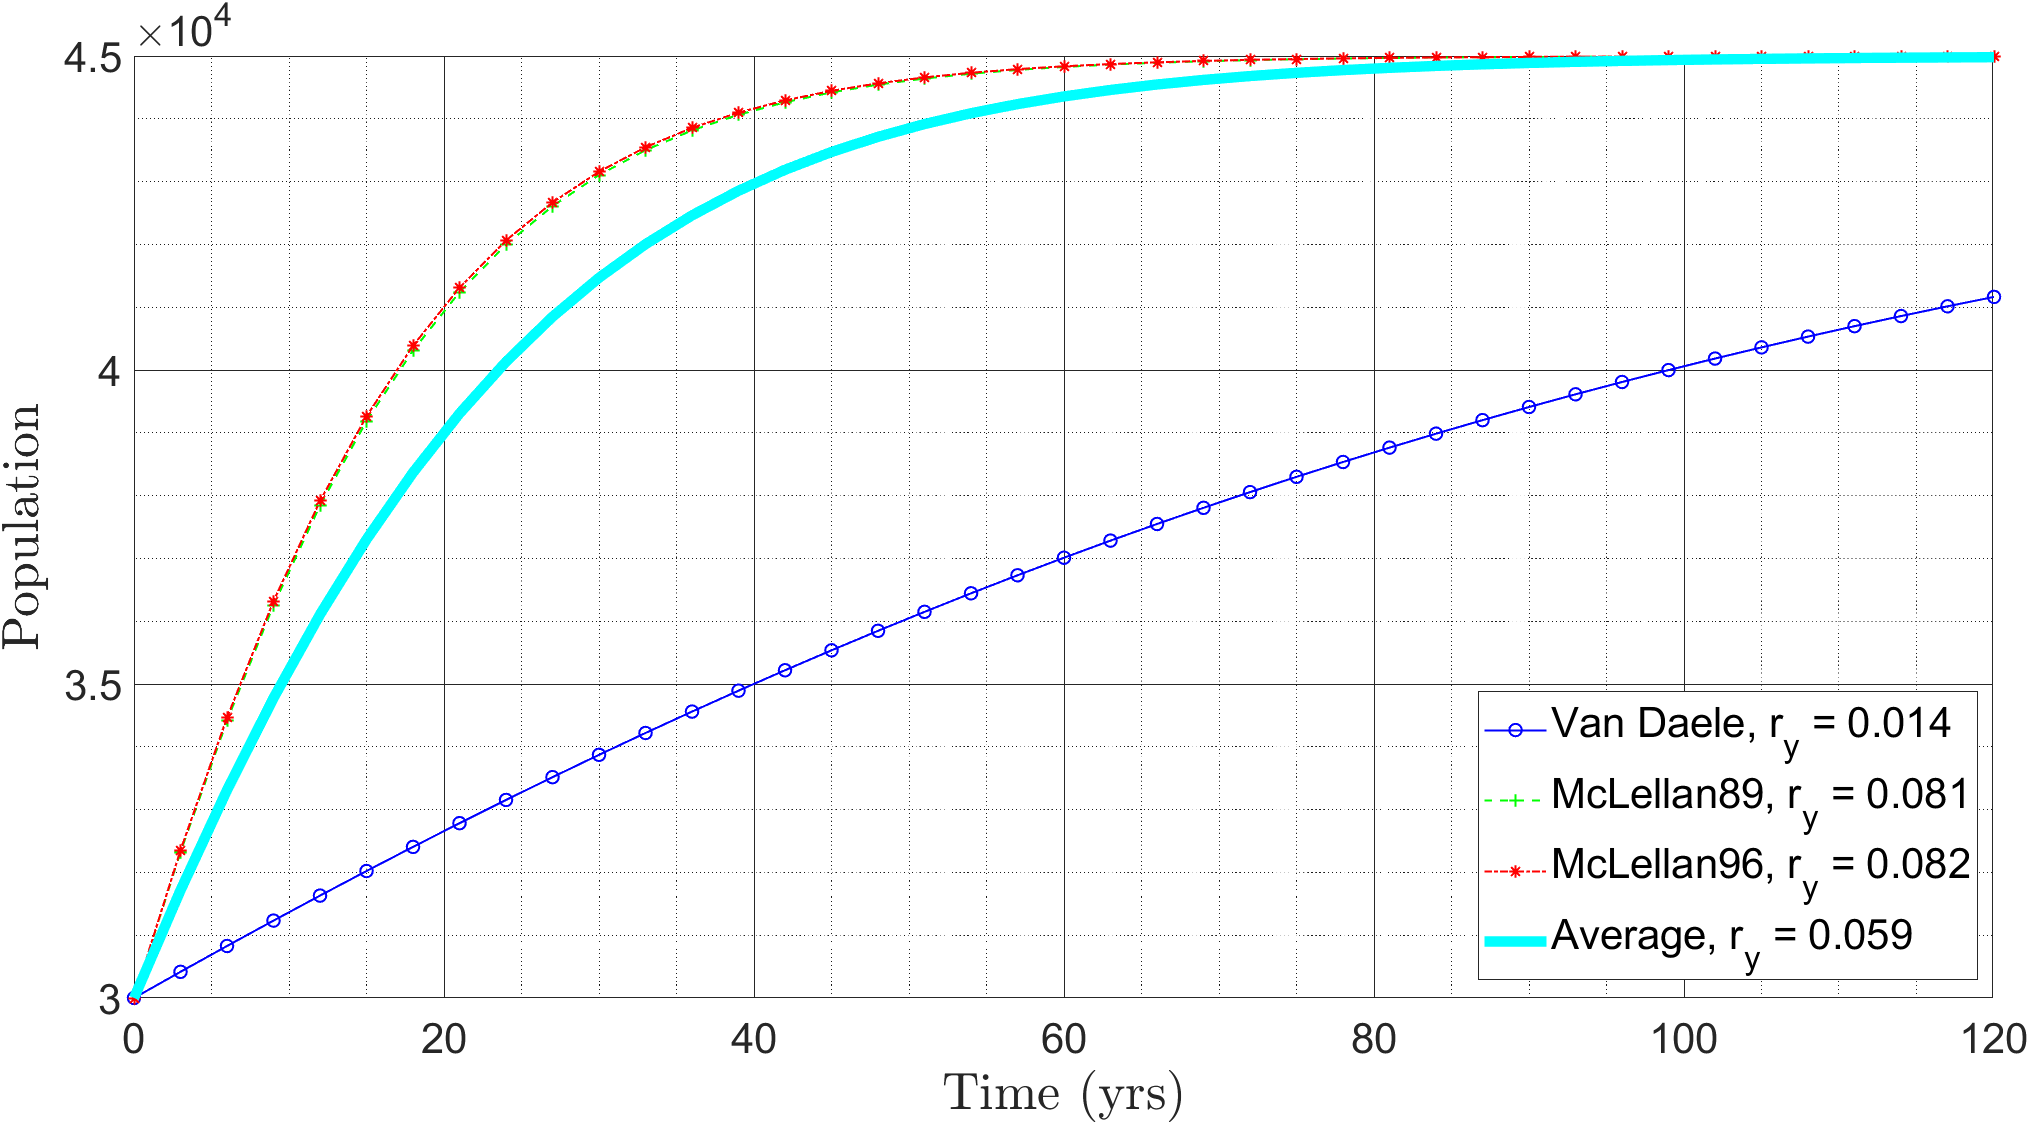
\includegraphics[width=14cm]{Pictures/Bear Pop/different growth rates.png}
\end{figure}
\begin{figure}[H]
    \centering
    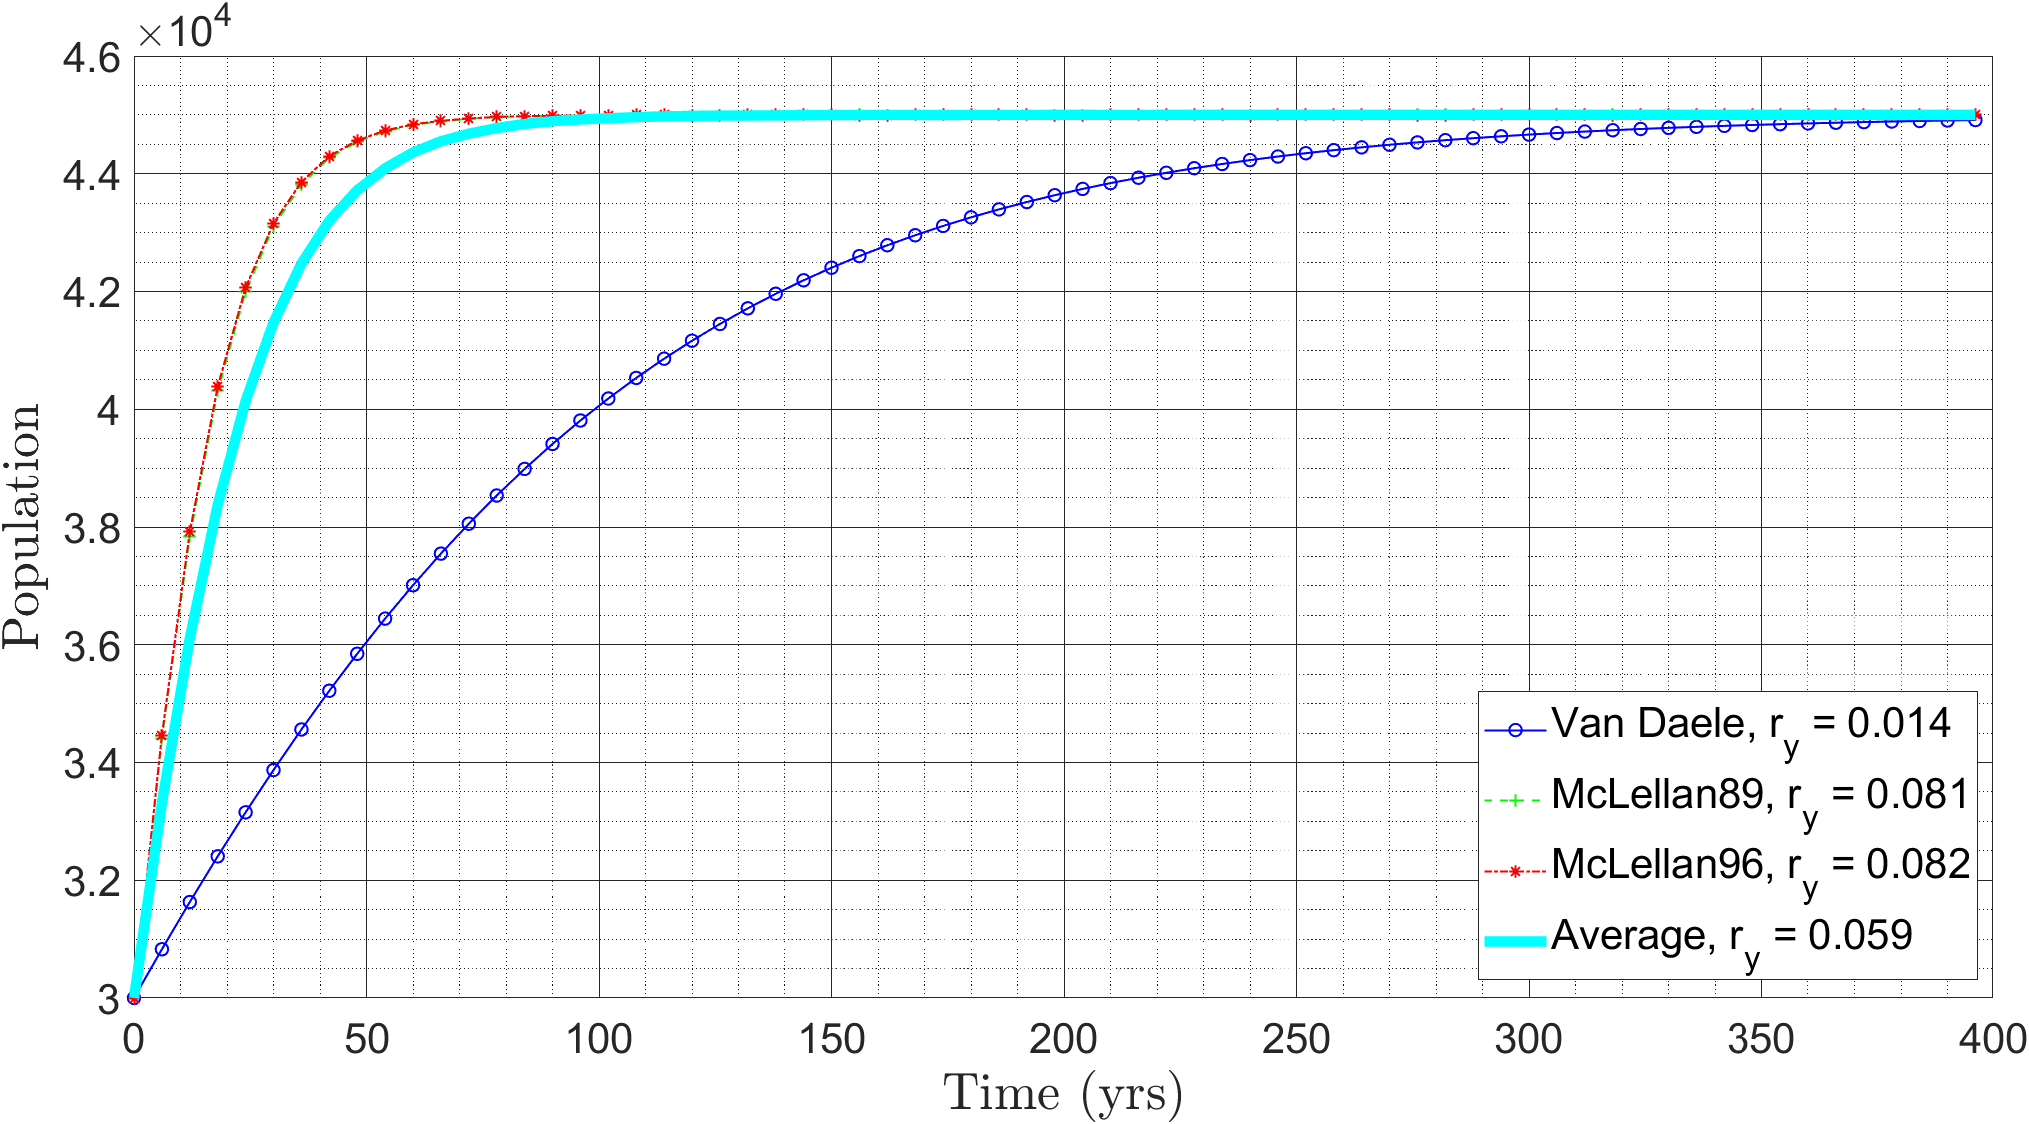
\includegraphics[width=14cm]{Pictures/Bear Pop/different growth rates large.png}
    \caption{\singlespacing
    Plots of the Alaskan brown bear logistic growth equation, \equationautorefname~\eqref{eq:LogBear}, for each of the growth rate parameter values, $r_y$, discussed in the articles above, as well as the average of all the growth rates. 
    The first graph represents a time span of 120 years, and the second represents 400 years.}
    
    % This figure displays the solutions of the logistic growth equation, \equationautorefname~\eqref{eq:LogBear}, for each of the growth rates, $r_y$, from each of the articles discussed above.
    % Also, the mean of all the growth rates is also substituted in the logistic growth model and illustrated with a bold line on the graphs.}
    \label{fig:LogGrowthTrials}
\end{figure}
In the plots above, McLellan's growth rates illustrate that the brown bear population will reach its environmental capacity within 80 years from an initial population of 30,000, while Van Daele's and Barnes' show that it would take the brown bears approximately 400 years.
For this thesis, we estimate the growth rate parameter for the brown bear population by calculating the mean of all the growth rates discussed earlier, resulting in an estimated value of $r_y=0.059$.
\figureautorefname~\ref{fig:LogGrowthTrials} shows that using this growth rate would result in the brown bears reaching their environmental limit in approximately 100 years.